\Problem{Connect}{connect}
% author: Jimmy M�rdell

\begin{wrapfigure}{r}{3cm}
\vspace{-5mm}
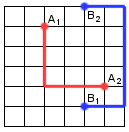
\includegraphics[width=\linewidth,keepaspectratio=true]{connect/connect}
\vspace{-9mm}
\end{wrapfigure}

\noindent
When constructing electric circuits one has to connect pairs of points using wire, preferable as short as possible.
In this problem we have an empty circuit board of size $N \times M$ where we want to connect the two points $A_1$ and $A_2$
with each other using one wire, and the two points $B_1$ and $B_2$ with each other using another wire.
The wires must go along the horizontal and vertical edges of the grid (see figure), and the two wires may not share a common vertex.
Determine the minimum length of wire needed to do so. The wire may not go outside the circuit board.

\Input
The first line contains two integers, $N$ ($2 \le N \le 100$) and $M$ ($2 \le M \le 100$), the grid size of the circuit board.\\
Then follows four lines containing the coordinates for the points $A_1$, $A_2$, $B_1$ and $B_2$, respectively. Each coordinate pair will be described using two integers and will correspond to an intersection point in the grid. The first coordinate will be between $0$ and $N$ inclusive and the second coordinate between $0$ and $M$ inclusive. All coordinate pairs will be unique.

\Output
A single line containing the minimum length of wire needed to connect the points, or "IMPOSSIBLE" if it's not possible to do so.

\Xample{connect/connect.1}

\Xample{connect/connect.2}
